\documentclass[11pt]{article}
\usepackage[margin=1in]{geometry}
\usepackage{graphicx}
\usepackage{amsmath}
\usepackage{caption}
\usepackage{subcaption}
\usepackage{float}
\usepackage{hyperref}

\title{Impact of Air Pollution on Respiratory Diseases}
\author{}
\date{}

\begin{document}
\maketitle

\section*{Introduction}
This report examines whether air pollution, specifically PM2.5 levels, impacts respiratory diseases. Using air quality and respiratory health data, we performed correlation and regression analyses to uncover potential links.

\section*{Analysis}

\subsection*{State-Level Analysis}
State-level data shows a moderate positive Pearson correlation (0.51) between PM2.5 levels and respiratory health metrics. However, an R\textsuperscript{2} score of 0.26 indicates PM2.5 alone explains only a small portion of the variation in respiratory outcomes. The regression trendline reflects a slight increase but lacks strong predictive power.

\begin{figure}[H]
    \centering
    \begin{subfigure}{0.48\textwidth}
        \centering
        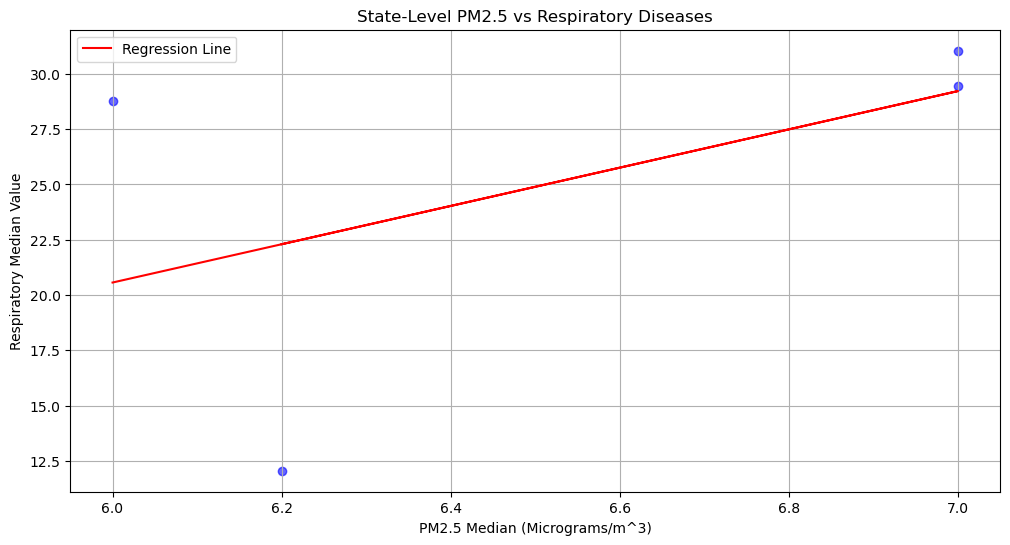
\includegraphics[width=\textwidth]{output_2_0.png}
        \caption{State-Level PM2.5 vs Respiratory Diseases}
    \end{subfigure}
    \hfill
    \begin{subfigure}{0.48\textwidth}
        \centering
        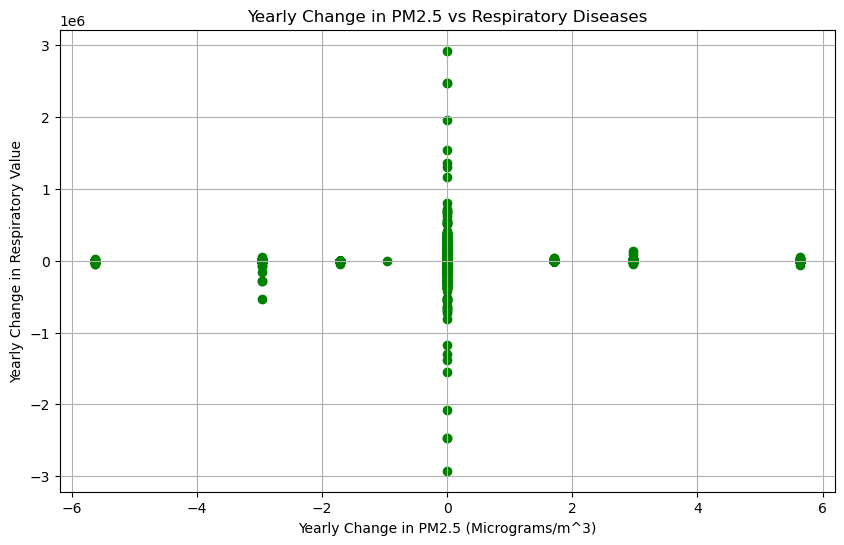
\includegraphics[width=\textwidth]{output_3_1.png}
        \caption{Yearly Change in PM2.5 vs Respiratory Diseases}
    \end{subfigure}
    \caption{State-Level and Yearly Changes Analyses}
\end{figure}

\subsection*{Distribution Analysis}
The distributions of PM2.5 levels and respiratory metrics exhibit considerable variability. The histograms below illustrate these patterns:

\begin{figure}[H]
    \centering
    \begin{subfigure}{0.48\textwidth}
        \centering
        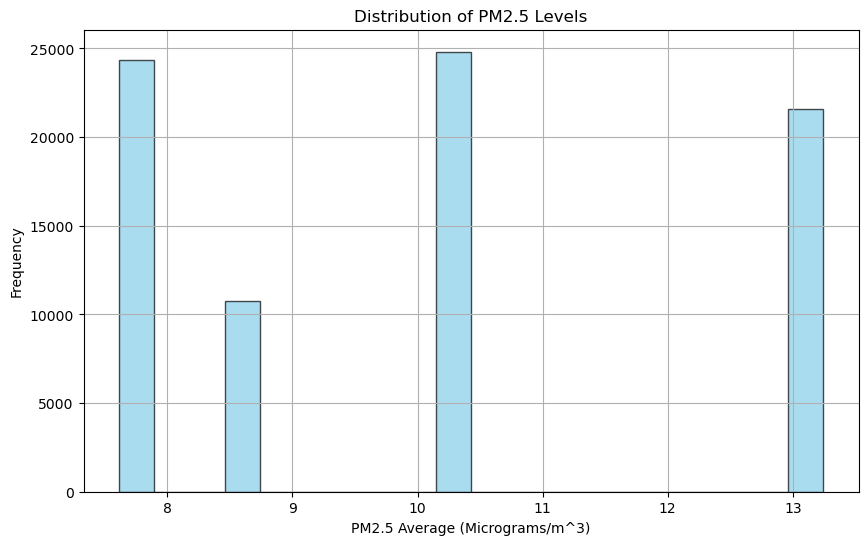
\includegraphics[width=\textwidth]{output_4_0.png}
        \caption{Distribution of PM2.5 Levels}
    \end{subfigure}
    \hfill
    \begin{subfigure}{0.48\textwidth}
        \centering
        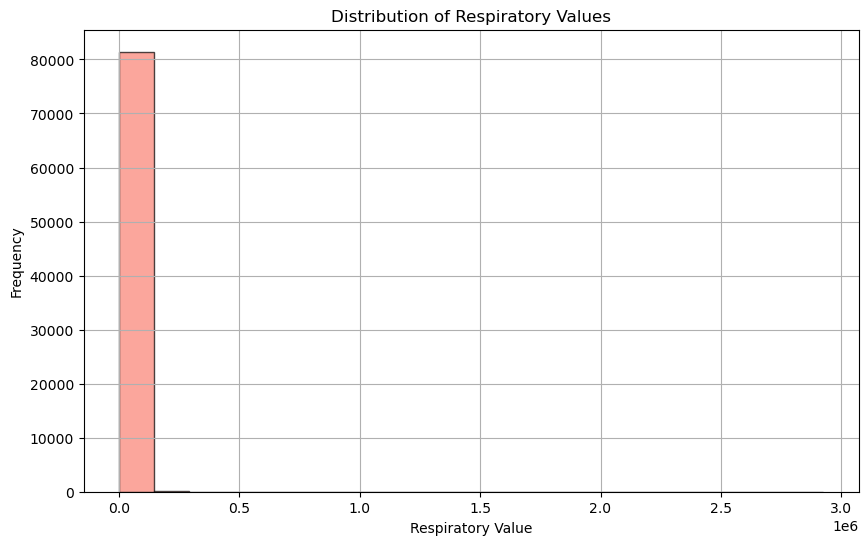
\includegraphics[width=\textwidth]{output_4_1.png}
        \caption{Distribution of Respiratory Values}
    \end{subfigure}
    \caption{Distributions of PM2.5 Levels and Respiratory Values}
\end{figure}

\subsection*{Trends Over Time}
State-level respiratory disease trends show year-to-year variation. The heatmap below captures these dynamics:

\begin{figure}[H]
    \centering
    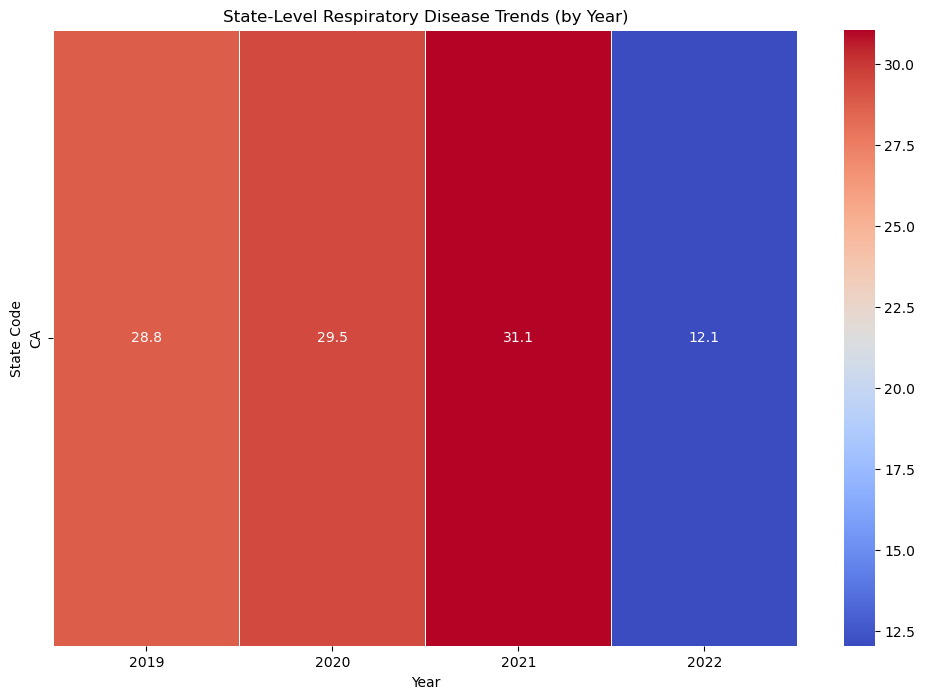
\includegraphics[width=0.8\textwidth]{output_5_0.png}
    \caption{State-Level Respiratory Disease Trends (by Year)}
\end{figure}

\subsection*{Pollutant Correlations}
Additional analysis of pollutants and respiratory health indicates weak correlations, as shown in the chart below:

\begin{figure}[H]
    \centering
    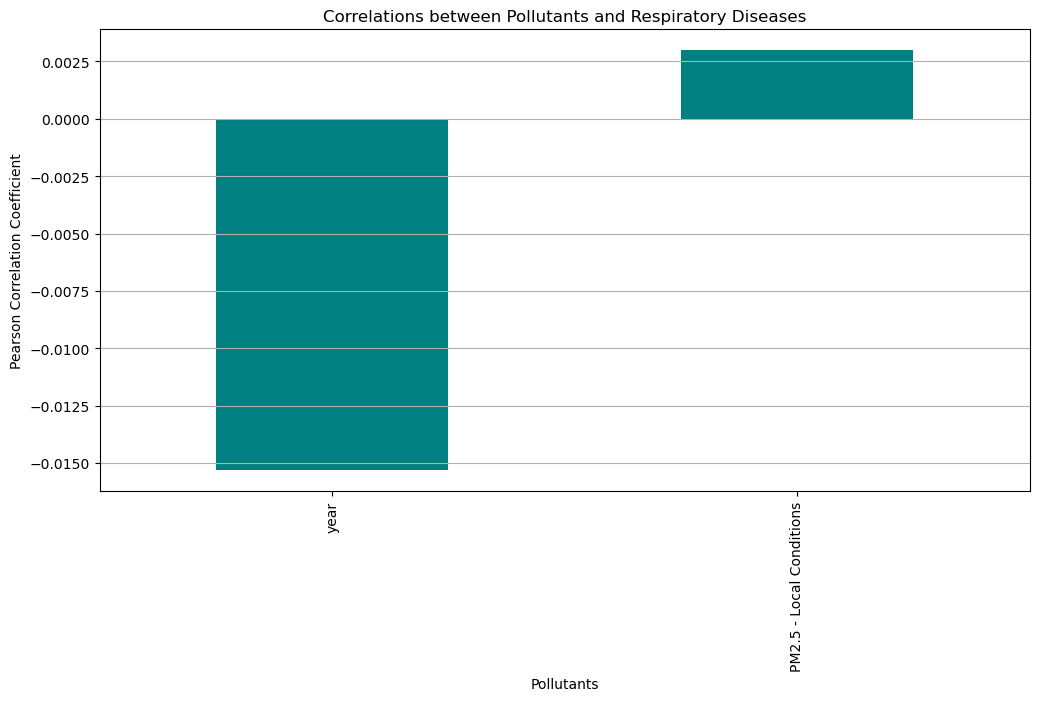
\includegraphics[width=0.8\textwidth]{output_6_1.png}
    \caption{Correlations between Pollutants and Respiratory Diseases}
\end{figure}

\section*{Conclusion}
The findings suggest a moderate association between PM2.5 levels and respiratory diseases at the state level, though with limited explanatory power (R\textsuperscript{2}). Yearly changes and county-level data provide no substantial evidence of direct impact. Improved datasets are essential for a more definitive understanding of air pollution's effects on respiratory health.

\section*{Data Sources and Pipeline}

\subsection*{Air Quality Data}
\textbf{Source:} \href{https://aqs.epa.gov/aqsweb/documents/data_api.html}{EPA Air Quality System (AQS)}  
\textbf{Reason for Selection:} Provides detailed PM2.5 pollution measurements across California, critical for understanding environmental health impacts.  
\textbf{Content:} Includes pollutant levels, sampling locations, dates, and measurement units.  
\textbf{Structure and Quality:}
\begin{itemize}
    \item Structured tabular data with attributes such as \texttt{state\_code}, \texttt{date\_local}, and \texttt{sample\_measurement}.
    \item Missing values handled during preprocessing.
    \item High reliability as data is maintained by the EPA.
\end{itemize}
\textbf{License and Obligations:}  
Licensed under open access by the EPA. Obligations include attribution, addressed in the project documentation.  
\href{https://data.gov/open-gov/}{License Details}

\subsection*{Respiratory Health Data}
\textbf{Source:} \href{https://data.cdc.gov/Chronic-Disease-Indicators/U-S-Chronic-Disease-Indicators/hksd-2xuw}{CDC Chronic Disease Indicators Dataset}  
\textbf{Reason for Selection:} Provides health metrics for respiratory conditions (e.g., asthma) at state and county levels.  
\textbf{Content:} Includes respiratory health indicators, demographic stratifications, and annual statistics.  
\textbf{Structure and Quality:}
\begin{itemize}
    \item Structured tabular data with fields such as \texttt{topic}, \texttt{state\_code}, \texttt{respiratory\_value}, and \texttt{year}.
    \item Data contains noise, requiring filtering for relevant indicators.
\end{itemize}
\textbf{License and Obligations:}  
Open Data license with attribution requirements, fulfilled via documentation.  
\href{https://opendatacommons.org/licenses/odbl/1-0/}{License Details}

\subsection*{Pipeline Overview}
The analysis pipeline is summarized below:

\begin{figure}[H]
    \centering
    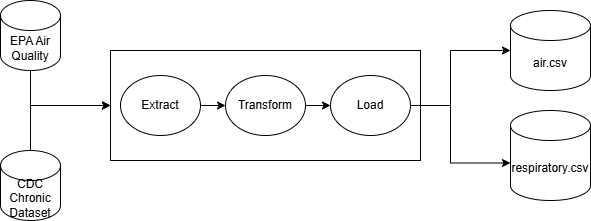
\includegraphics[width=0.8\textwidth]{pipeline.png}
    \caption{Data Processing Pipeline}
\end{figure}

\textbf{Implementation Highlights:}
\begin{itemize}
    \item \textbf{Multithreading:} Data extraction, transformation, and loading were performed in parallel to reduce runtime.
    \item \textbf{Modular Design:} The project codebase is organized into modules, ensuring clear segregation of responsibilities:
    \begin{itemize}
        \item \texttt{extract.py}: Extracts raw data from sources.
        \item \texttt{transform.py}: Cleans and processes the extracted data.
        \item \texttt{load.py}: Saves the transformed data for analysis.
    \end{itemize}
    \item \textbf{Reproducibility:} The modular approach ensures each step is well-documented, tested, and easily reproducible.
\end{itemize}

\end{document}
